\section{User Stories}

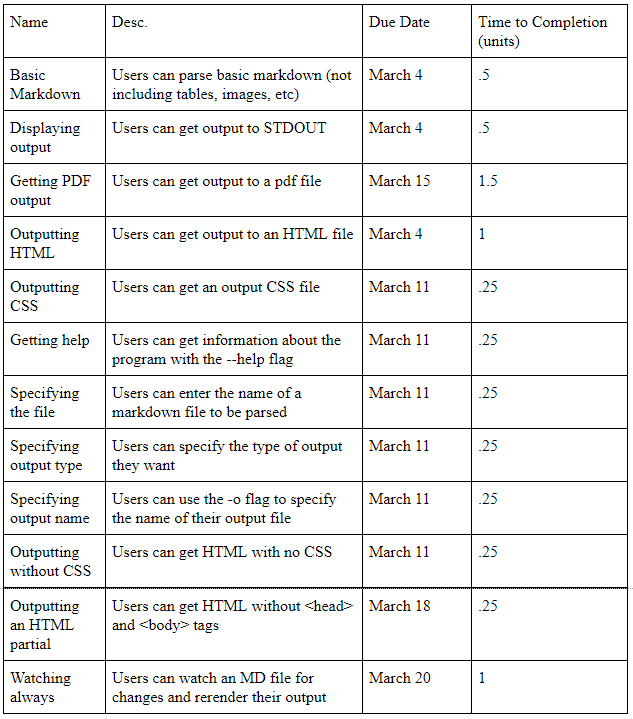
\includegraphics[width=400pt]{images/UserStoriesTable.png}

%1 --> Basic Markdown
\subsection{Basic Markdown}
This user story requires us to create the mddata class type, read in files, and 

%2 --> Displaying Output
\subsection{Displaying Output}
This user story just requires us to format the mddata object in a way that can be printed to the screen.
We plan on making objects go on their own lines, with a character at the start of the line indicating what type of object it is.

%3 --> Getting PDF output
\subsection{Getting PDF Output}
For this section, we performed a spike because we were not familiar specifically with the PDF format.

To do this spike, we built up a PDF file manually to simulate creating one programmatically. This was very difficult. PDF does not automatically create line breaks for text, so it is necessary for the user to determine when to break lines based on the size of the characters that appear on the line; in a non-monospace font, this means tracking the size of every character used in the font. PDF also uses a linked list data structure at the end of the document that stores a reference to every PDF object that appears in the document; to use this properly we would likely have to develop another data structure to store each PDF object we created as we wrote the document.

In conclusion, while writing PDF output is possible, it may not be technically feasible in the time frame that we have for this project, so we may need to focus only on generating HTML output.

%4 --> Outputting HTML
\subsection{Outputting HTML}
For this user story, we will need to iterate over our mddata data type, and construct HTML elements from each subclass within our data. This will then need to go to an HTML file.

%5 --> Outputting CSS
\subsection{Outputting CSS}
To output a file in HTML with CSS styling, when the user gives their file, they will also provide a CSS link. So, first the markdown file will be sent to be parsed into C++ data. This data will then return to the command line interface that would then send it to be converted into the HTML data. Then again this data will be returned to the command line interface. This time when the HTML data is sent out to the output, it will also contain the CSS styling referense that the user had initially provided.  
\hspace{-5cm}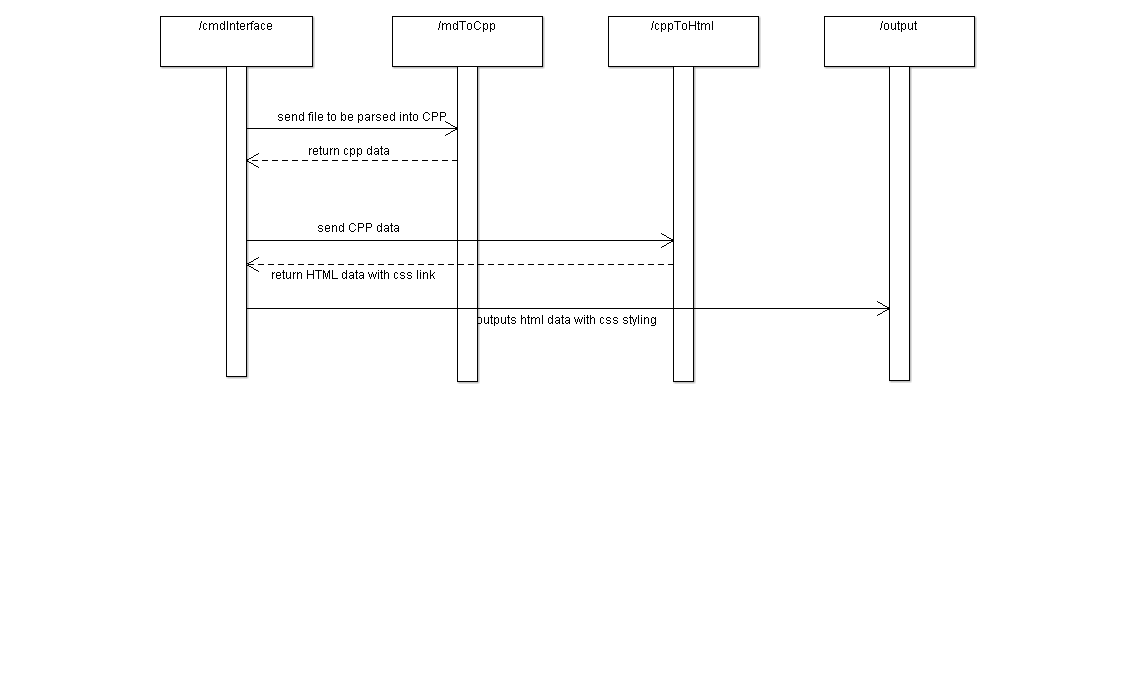
\includegraphics[width=700pt]{images/Output.png}

%6 --> Getting Help
\subsection{Getting Help}
If the user is unsure of how to use the program, they can request help by typing the flag '--help'. The command line interface would then take this in and return the instructions of how to use the program. This would include the flags that specify HTML output, C++ data output, standard out output, and pdf output. Additionally, it will show them the flags used to specify the name of the file that they want thier markdown to be converted and stored into. 
\hspace{-2cm}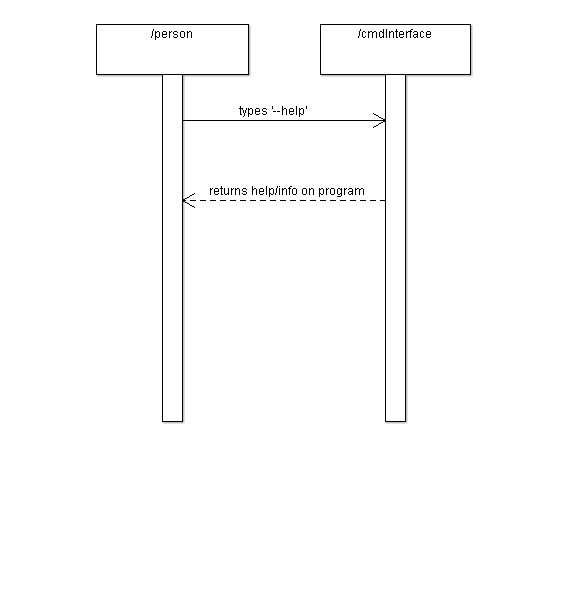
\includegraphics[width=450pt]{images/GettingHelp.png}

%7 --> Specifying the File
\subsection{Specifying the File}
The user needs to provide a markdown file and so they enter the name of the file then the command line interface searches for the file and sends it to be converted into the c++ data, which starts the whole conversion process.
\hspace{-2cm}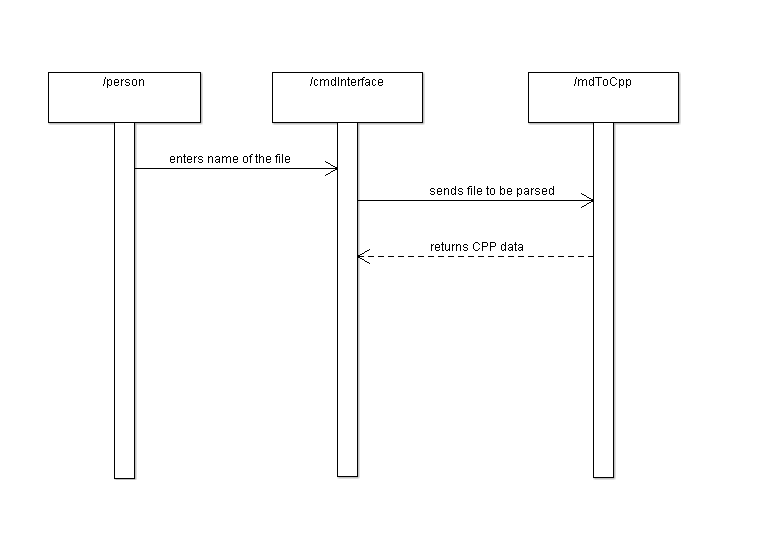
\includegraphics[width=500pt]{images/SpecifyingFile.png}

%8 --> Specifying the Output Type
\subsection{Specifying the Output Type}
The user has different options of what to do with their file. They could have thier markdown be parsed into pdf data or html (both of which require it to be converted into C++ data first). To do this, if the user wants an html file, they would enter the flag: '--html' after their markdown file name. This would cause the command line to send the markdown file to be converted into c++ data and then send it back to the command line which would send it to be converted into HTML data, since that was the flag that the user specified. The only difference if the user wanted pdf would be the flag: '--pdf' then after the markdown is parsed into c++, it would be sent to be parsed into pdf data, as per user request.
\hspace{-3cm}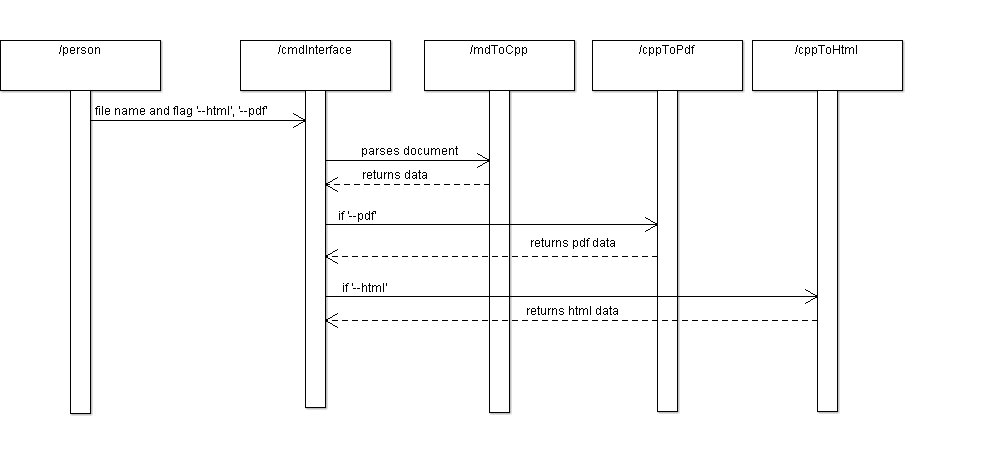
\includegraphics[width=550pt]{images/SpecifyingOutputFile.png}

%9 --> Specifying the Output Name 
\subsection{Specifying the Output Name}
If the user would like to specify what they want their new file representing thier markdown data to be called, they could do this by entering the name of desired file after their markdown file name. This would then be sent to the command interface and then to the markdown to c++ class to store the name for future retrieval. It would also be outputted under this name.
\hspace{-3cm}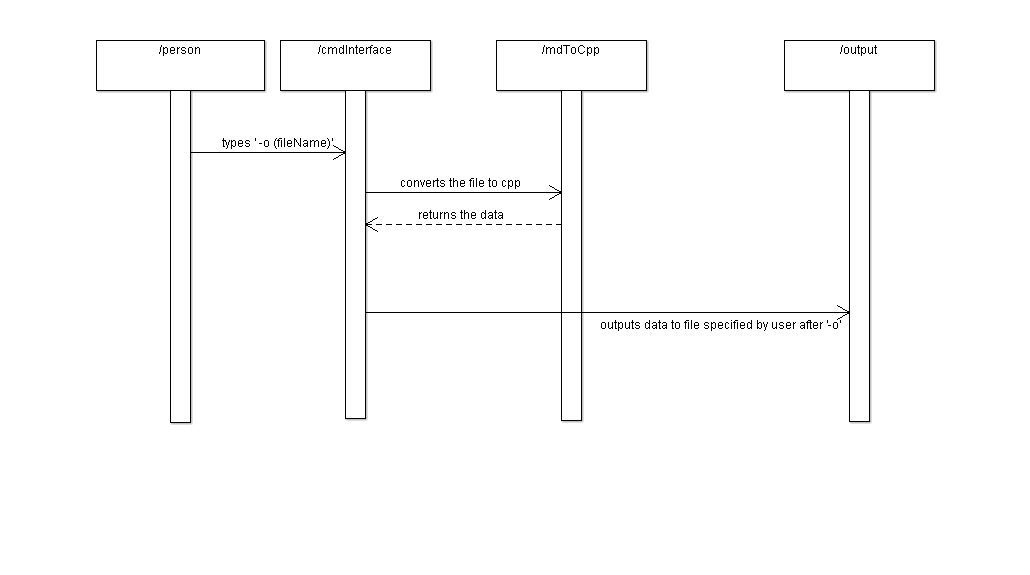
\includegraphics[width=500pt]{images/SpecifyingOutputName.png}

%10 --> Outputting without CSS
\subsection{Outputting without CSS}
For this section, the project can allow user to get HTML file without CSS. This section expect to be finished on March 11, it requires the previous units to prase Markdown data into HTML file, the Outputting HTML task.

%11 -->    Outputting an HTML partial
\subsection{Outputting an HTML partial}
For this section, the project can allow user to get HTML file without head and body tags. This section expect to be finished on March 18, it requires the previous units to prase Markdown data into HTML file, the Outputting HTML task.

%12 --> Watching always
\subsection{Watching always}
This section allow user to review the markdown for making changes and rerender a new output the user want.
